\section{Evaluation}
To demonstrate the effectiveness of our method, we evaluate our transfer learning based classification technique on actual data and point names of sensors from three commercial buildings. Extensive experiments demonstrate that our technique is able to accurately classify by type for a considerable portion of examples without human intervention. We also discuss how the threshold parameter $\delta$ on similarity score affect the learning accuracy and also explain the decision of how to set such a parameter.

\subsection{Taxonomy and Data Collection}
\begin{figure}[t]
\centering
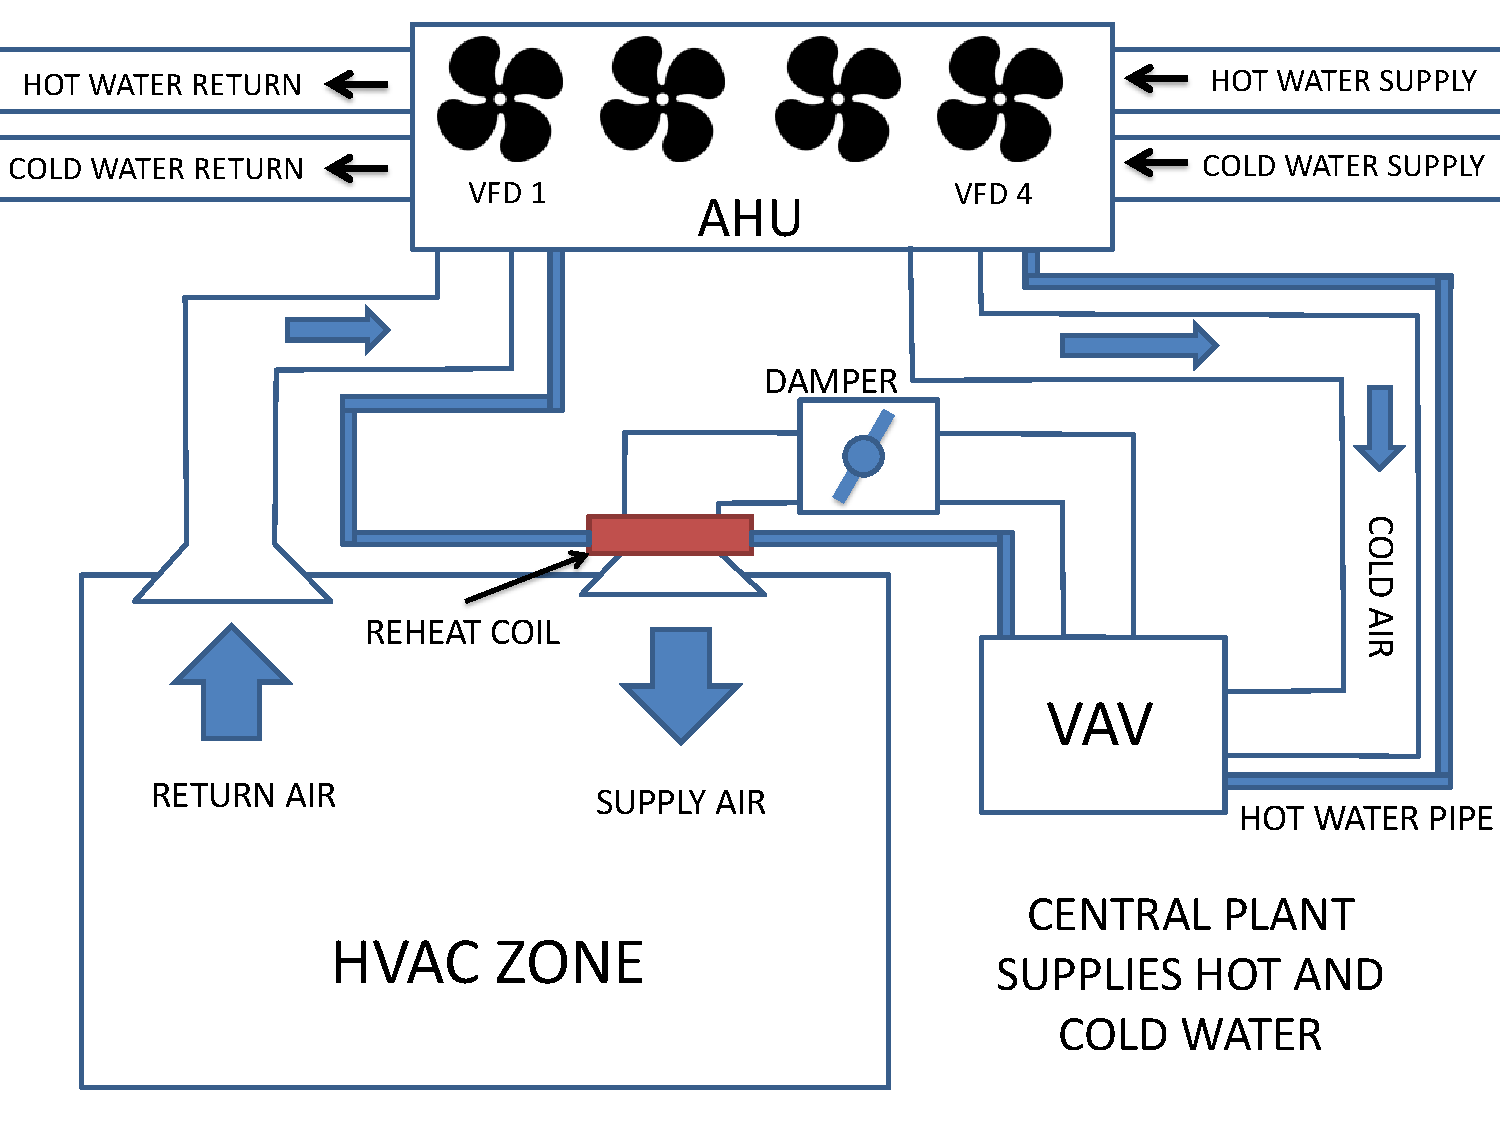
\includegraphics[width=0.38\textwidth]{./fig/hvac}
\caption{A typical HVAC system consisting of an air handler unit (AHU), several variable air volume boxes (VAV), water-based heating/cooling pipes and air circulation ducts. (Figure used with permission from the authors of~\cite{sentinel}.)}
\label{fig:hvac}
\end{figure}

Figure~\ref{fig:hvac} illustrates a typical heating, ventilation, and air conditioning (HVAC) system deployed in modern commercial buildings. 
An HVAC system usually uses a combination of hot and cold water pipes in conjunction with
air handler units (AHU) to maintain the appropriate thermal environment within the building.
An HAVC system usually consists of several AHUs and each AHU is responsible for a physical zone
in the building. An AHU consists of variable speed drives that supply cold air
(cooled by the supplied cold water) using ducts to VAV boxes distributed throughout the building.
The hot water loop is also connected to these VAV boxes using separate pipes. Each VAV box
controls the amount of air to be let into an HVAC zone using dampers, whose opening angle
can be programmed. A reheat coil, which uses supplied hot water, is used to heat the air to
meet the appropriate HVAC settings for each zone.

Table~\ref{table:num} summarizes all the types of sensors evaluated in our analysis in these three buildings and the number of sensors of each type. ``Room temperature'' measures the temperature in room and for a better understanding, all the other temperature measurements on water circulation and air ventilation are illustrated in Figure~\ref{fig:hvac}. For setpoints, we assign only
one general type which includes all set points for every actuator configured in the building.

Our evaluation data set containing both data and point names of sensor streams is collected from over 2,500 sensors of different types deployed in three commercial buildings. 
We collected a week's worth of data from each building.
Specially, Building A is the Rice Hall at the University of Virginia, where the sense points report to a database by Trane anywhere between every 10 seconds to every 10 minutes.
Both building B and C are from UC Berkeley: B is the Sutardja Dai Hall with sensors and equippment from KETI~\cite{keti} and Siemens~\cite{bacnet}, while building C is the Soda Hall what uses an archaic system by Barrington Controls which is no longer in business. 
Points and sensors in these two buildings transmit data to an archiver~\cite{smap} periodically from anywhere between every 5 seconds to every 10 minutes.


\begin{table}[t]
\centering
\begin{tabular}{l | l l l}
\hline
& \multicolumn{3}{c}{Building} \\
Type & A & B & C\\
\hline\hline
$CO_{2}$ & 16 & 52 & 0\\
Humidity & 54 & 52 & 0\\
Air Pressure & 142 & 216 & 215\\
Room Temp & 159 & 231 & 208\\
Facility Operation Status & 59 & 72 & 41\\
Facility Control & 0 & 138 & 403\\
Setpoint & 140 & 486 & 229\\
Air Flow Volume & 14 & 172 & 9\\
Damper Position & 0 & 290 & 10\\
Fan Speed & 0 & 25 & 15\\
HW Supply Temp & 27 & 1 & 0\\
HW Return Temp & 15 & 1 & 0\\
CW Supply Temp & 18 & 2 & 11\\
CW Return Temp & 15 & 3 & 10\\
Supply Air Temp & 20 & 17 & 3\\
Return Air Temp & 6 & 2 & 4\\
Mixed Air Temp & 5 & 2 & 3\\
Ice Tank Entering Temp & 1 & 2 & 0\\
Ice Tank Leaving Temp & 1 & 4 & 0\\
Occupancy & 25 & 52 & 0\\
Timer & 0 & 0 & 15\\ \hline
Sum & 575 & 1124 & 1166\\ \hline
\end{tabular}
\caption{Number of points by type for the 3 test buildings. ``Temp" stands for ``temperature", ``HW" for ``hot water" and ``CW" for ``cold water".}
\label{table:num}
\end{table}


All of our learning and classification processes are implemented based on the scikit-learn~\cite{scikit} library, which is an open-source machine learning package 
implemented mostly in Python providing a rich set of APIs.

\subsection{Base Classifiers and Baseline}
\label{sec:baseline}
Our transfer learning based approach exploits a few base classifiers. Each base classifier will be trained on the same set of data features from the source building in a general way, therefore there is no particular requirement on what classifiers should be selected here.
Particularly, we employ three base classifiers: Ranfom forest, linear regression and support vector machines with RBF kernels.


\begin{figure*}[ht!]
\centering
  \begin{subfigure}{0.32\textwidth}
                \centering
    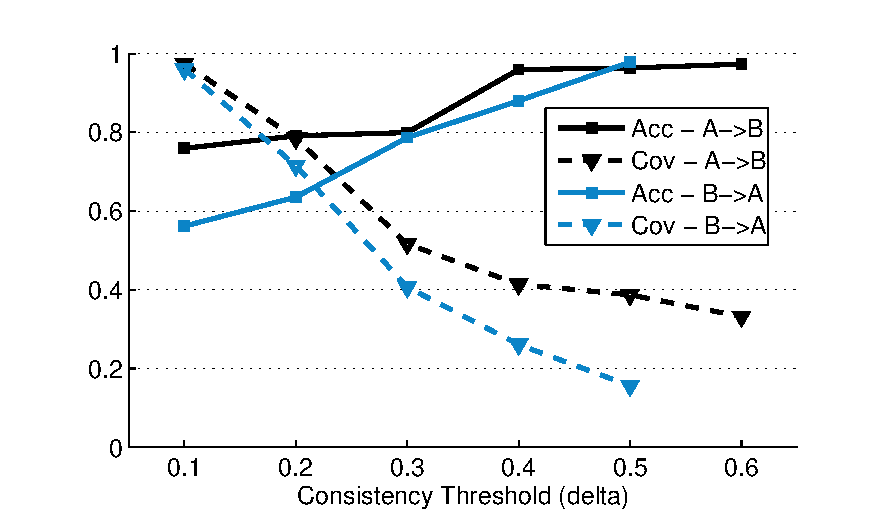
\includegraphics[width=\textwidth]{./fig/TL_AB.eps}
                \caption{A and B}
  \end{subfigure}
  \begin{subfigure}{0.32\textwidth}
                \centering
    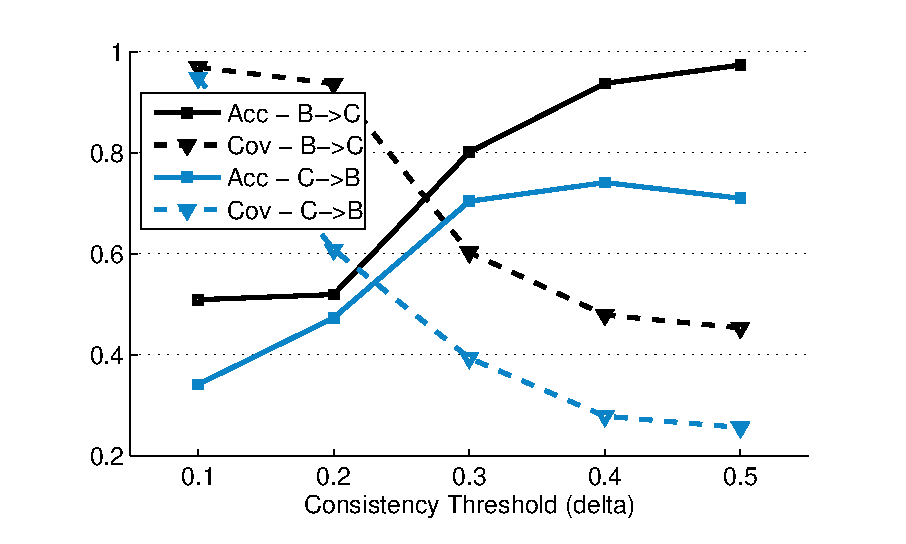
\includegraphics[width=\textwidth]{./fig/TL_BC.eps}
                \caption{B and C}
  \end{subfigure}
  \begin{subfigure}{0.32\textwidth}
                \centering
    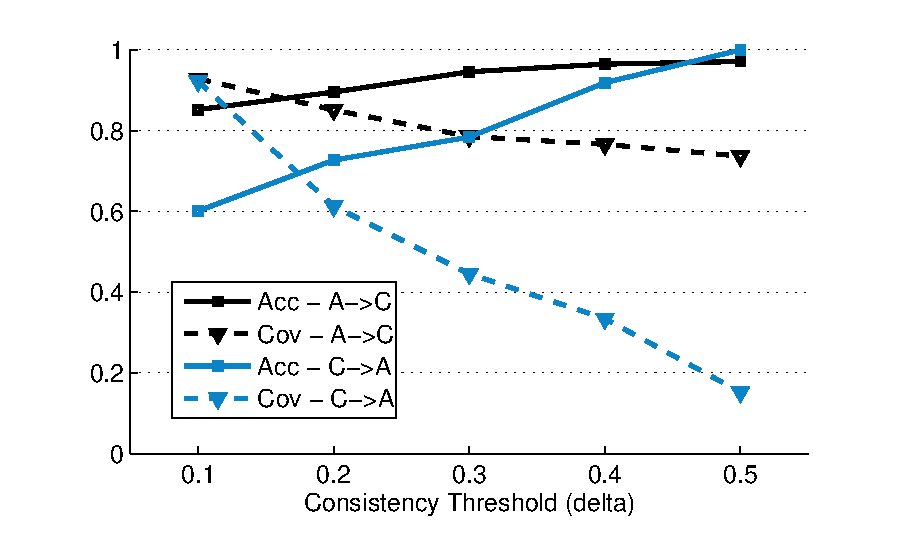
\includegraphics[width=\textwidth]{./fig/TL_AC.eps}
                \caption{A and C}
  \end{subfigure}
\caption{Type classification accuracy against labeled percentage with transfer learning between different pairs of buildings.}
\label{fig:tl_acc}
\end{figure*}


As a baseline to compare our proposed approach against, we adopt a 


For classification, we measure the averaged cross-validation accuracy in two different scenarios (intra- and inter- buildings). In the intra-building case, the 
data from a single building is split into training and testing sets, where the results illustrate how accurately the type information can be inferred using local 
within-building information. For inter-building case, the experiment performs training and testing across buildings, i.e, train the classifier on the data from building A 
and test it on building B.  
This set of experiments tests how well we can apply the classification boundaries from one building and apply it to another.

\subsection{Base Classifier Performance}


\subsection{Transfer Learning Accuracy}
We run the two sets of experiments described above, i.e, the intra- and inter- building tests, to examine the effectiveness of feature design and measure how well 
the classifier performs. The classification results are summarized from Table~\ref{table:rice}-\ref{table:sdh_x}. %,~\ref{table:sdh},~\ref{table:rice_x},~\ref{table:sdh_x}.
In the table, each row is specific to a \emph{type} and each column is the \emph{percentage} of the full data set that was used for training.
Each cell shows two values.  The value without parentheses is the average classification accuracy for the richer feature-vector. 
The value in parentheses is the average classification accuracy for the approach described in 
Section~\ref{sec:baseline}. These are compared throughout the table.
The last column summarizes ``leave-one-out'' cross-validation\footnote{In LOO cross validation, each training set takes all the instances except one with the test set being 
the sample held out.} results for each approach.

\subsection{Exploitation of Labels in the New Building}
